\documentclass[10pt]{beamer}

\usetheme{CambridgeUS}
\usecolortheme{default}

\usepackage[utf8]{inputenc}
\usepackage{graphicx}
\usepackage{listings}
\usepackage{xcolor}
\usepackage{bm}
\usepackage{amsmath}
\usepackage{array}
\usepackage{url}
\usepackage{hyperref}

\graphicspath{{images/}}


\title{JPEG Compressor}
\author{Suciu Andrei}
\date{May 2025}


\hypersetup{
    pdftitle={IP Project},
    pdfauthor={Suciu Andrei},
    pdfsubject={JPEG Compressor},
    pdfkeywords={JPEG, compression, image processing}
}

\lstset{
    language=C,
    backgroundcolor=\color{black!80},
    basicstyle=\color{white}\ttfamily,
    keywordstyle=\color{orange}\bfseries,
    stringstyle=\color{green},
    commentstyle=\color{gray}\itshape,
%     numberstyle=\color{blue},
    identifierstyle=\color{white},
    directivestyle=\color{green}\bfseries,
    numbers=left,
    numbersep=5pt,
    tabsize=4,
    showspaces=false,
    showstringspaces=false,
    showtabs=false,
    breaklines=true,
    breakatwhitespace=true,
    frame=single,
    rulecolor=\color{white},
    xleftmargin=2em,
    framexleftmargin=1.5em,
    moredelim=[is][\color{blue}]{@}{@},
    literate=
        {0}{{{\color{blue!80}0}}}1
        {1}{{{\color{blue!80}1}}}1
        {2}{{{\color{blue!80}2}}}1
        {3}{{{\color{blue!80}3}}}1
        {4}{{{\color{blue!80}4}}}1
        {5}{{{\color{blue!80}5}}}1
        {6}{{{\color{blue!80}6}}}1
        {7}{{{\color{blue!80}7}}}1
        {8}{{{\color{blue!80}8}}}1
        {9}{{{\color{blue!80}9}}}1
}
\begin{document}

\begin{frame}
    \setlength{\parindent}{0pt}
%     \begin{titlepage}
        \begin{center}
            \vspace{0.2cm}
            \textbf{\large Department of Computer Science} \\[0.2cm]
            \textbf{\large Technical University of Cluj-Napoca} \\[0.2cm]
            
\includegraphics[width=1\textwidth]{utLogo.png} \\[0.5cm]

            \textbf{JPEG Compression} \\
            \textit{Laboratory activity 2025} \\[0.5cm]

            Student: Suciu Andrei \\
            Group: 30431 \\
            Email: suciu.se.an@student.utcluj.ro\\[1cm]

            \vfill

            Image Processing \\[0.2cm]
            
\includegraphics[width=1\textwidth]{utLogo.png} \\[0.2cm]


        \end{center}
%     \end{titlepage}
\end{frame}

\begin{frame}
 \tableofcontents
\end{frame}

\section{Introduction}

\begin{frame}{JPEG Compression}
    \centering{\huge{The JPEG Standard}}
    \vspace{20pt}
    \begin{itemize}
     \item JPEG is a widely used image compression standard developed during the 1980s and published in 1992 by the \textbf{Joint Photographic Experts Group}.
     \item JPEG is a \textbf{lossy} image compression method. It takes advantage of the \textbf{DCT} (Discrete Cosine Transform) to encode images.
     \item It is the most common format for storing and transmitting images  the internet.
    \end{itemize}

\end{frame}

\begin{frame}{The JPEG Codec}

    Although a JPEG file can be encoded in various ways, most commonly it is done with the standard JFIF encoding. This process consists of several steps:
    \begin{enumerate}
     \item The format of the image is converted from $\bm{RGB}$ to  $\bm{Y'C_bC_r}$ representing $\bm{Luminance}$, $\bm{Chroma\ Blue}$, and $\bm{Chroma\ Red}$ respectively.
     \item The resolution of the chroma channels is reduced, by a factor of 2 or 3. This reflects the fact that the eye is less sensitive to fine color changes than to brightness changes.
     \item The channels are split into blocks of $8\times8$ pixels, and for each block, the \textbf{Discrete Cosine Transform} is applied.
     \item Each of the blocks is \textbf{quantized}, ie. divided using a common \textbf{Qunatization Table}, dependent on the quality setting.
     \item The resulting blocks are further compressed with a lossless algorithm such as \textbf{Run Length Encoding} or \textbf{Huffman Encoding}.
    \end{enumerate}

\end{frame}


\section{Project Overview}

\begin{frame}{Project Overview}
    \begin{itemize}
     \item This project implements the JPEG codec for lossy compression/decompression
     \item This example will not use \textbf{Huffman Encoding} for the final compression step
     \item The project comes with associated headers for reading/writing \textbf{.BMP} and the final \textbf{.SAMS} binary files
     \item The program was written for \textbf{Linux} systems and must be compiled using the math and threads libraries
     \item For help, run the command with the \texttt{-h|--help} flag
    \end{itemize}
\end{frame}


\section{Color Space Conversion}

\begin{frame}{RGB to YCbCr conversion}
    \begin{itemize}
     \item \textbf{RGB} color space represents colors as combinations of Red, Green, and Blue components
     \item $\bm{Y'C_bC_r}$ separates luminance (brightness) from chromiance (color information)
     \item This separation allows for more efficient compression, since human vision is less sensitive to chromatic changes

     \vspace{0.5cm}
     \textbf{Conversion Formulas:}
     \begin{align}
      Y &= 0.299\cdot R + 0.587\cdot G + 0.114\cdot B\\
      C_b &= -0.169\cdot R - 0.331\cdot G + 0.5\cdot B + 128\\
      C_r &= 0.5\cdot R - 0.419\cdot G - 0.081\cdot B + 128
     \end{align}
    \end{itemize}
\end{frame}

\begin{frame}{Chroma Subsampling}

    \begin{figure}[h]
        \centering
        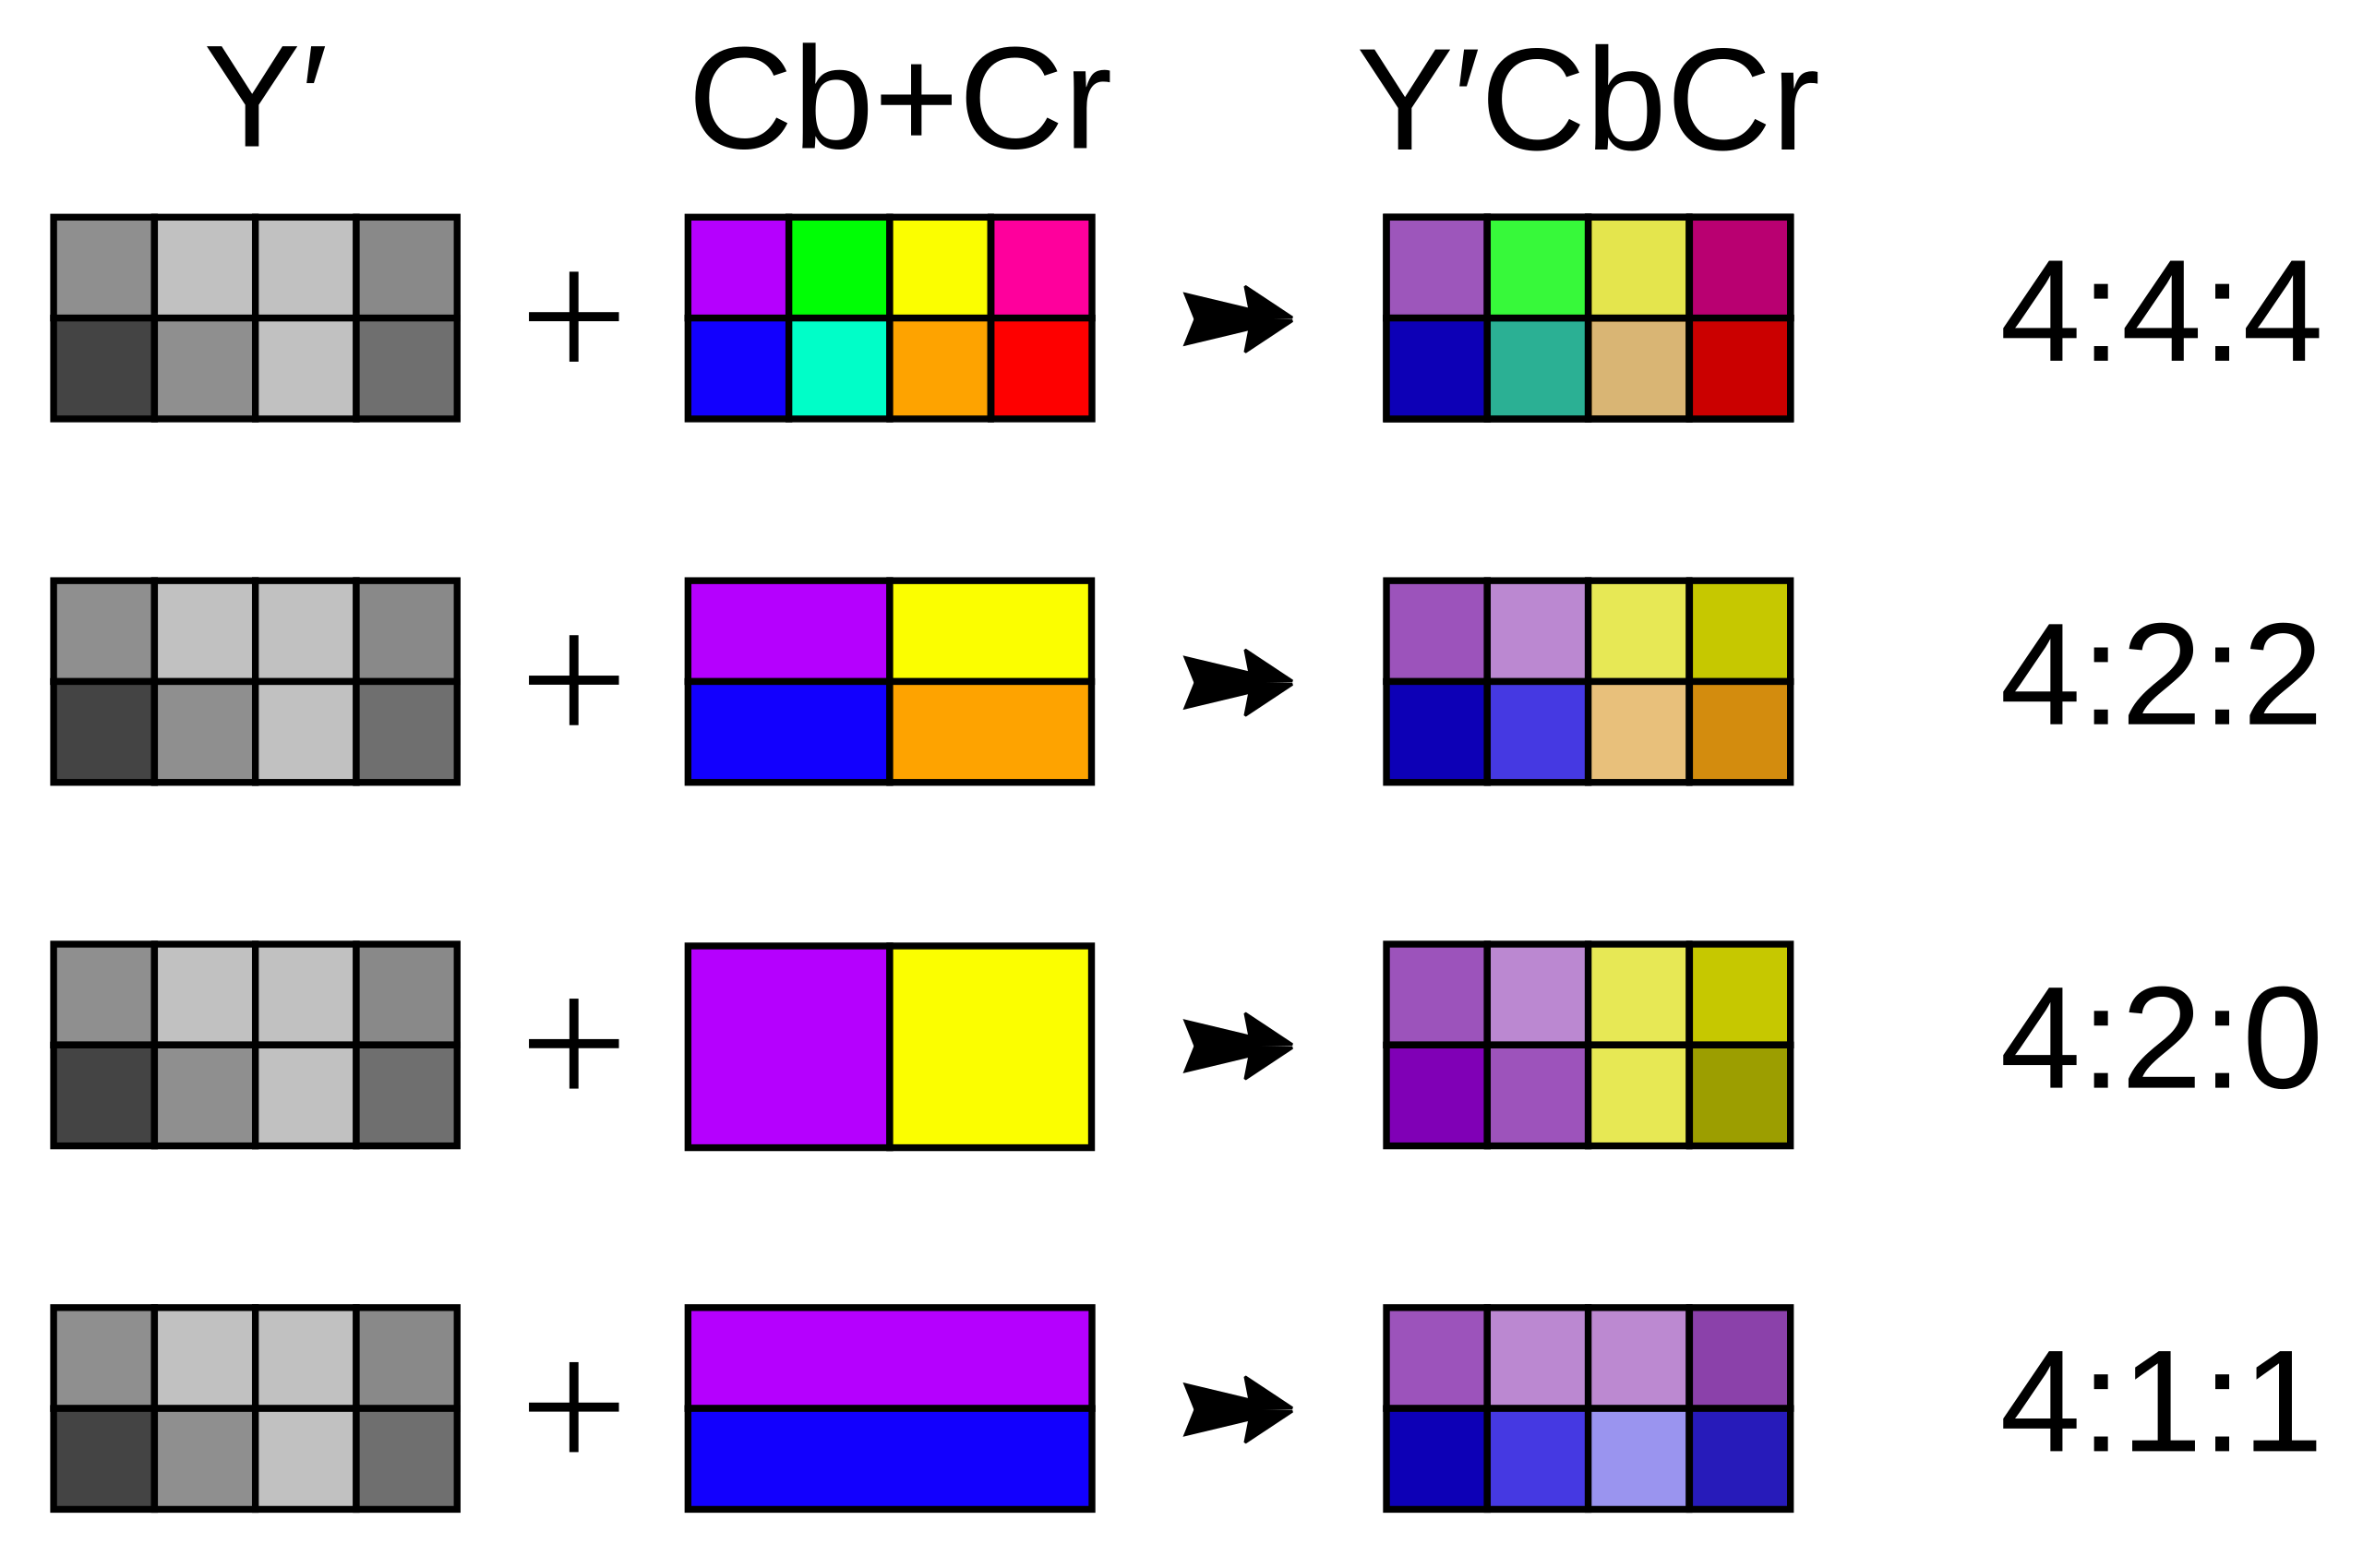
\includegraphics[width=0.3\textwidth]{chroma.png}
        \caption{Chroma Subsampling Examples}
    \end{figure}

    \begin{itemize}
     \item Human sight is less sensitive to color variations than brightness variations
     \item This allows us to reduce the resolution of the chroma channels without significant quality loss
     \item The most common subsampling strategy (4:2:0) is to reduce the resolution of the chroma channels by a factor of 2 both horizontally and vertically
     \item This results in $75\%$ less chroma data
    \end{itemize}

\end{frame}

\section{Block Division and DCT}

\begin{frame}{$8\times8$ Block Division}
    \begin{itemize}
     \item Each color channel is divided into non-overlapping $8\times8$ pixel blocks
     \item If image dimensions are not multiples of 8, padding is applied -- for the luminance channel, the previous value is replicated, and for chroma, a neutral 128 is used
     \item Each block is processed independently
     \item This approach allows for faster processing and localized compression
    \end{itemize}
\end{frame}

\begin{frame}{Discrete Cosine Transform (DCT)}
    \begin{itemize}
     \item DCT converts spatial domain data to frequency domain
     \item This concentrates block data in fewer coefficients (upper-left corener)
     \item The DC coefficient (top-left) represents average value of the block
     \item The AC coefficients (rest of the values) represent frequency components from low to high
    \end{itemize}

    \vspace{1cm}
    \textbf{2D DCT Formula:}
    \begin{small}
     $$\text{DCT}(i,j) = \frac{1}{4}C(i)C(j)\sum_{y=0}^{7}\sum_{x=0}^{7}\text{pixel}(y,x) \cdot \cos\left(\frac{(2y+1)i\pi}{16}\right) \cdot \cos\left(\frac{(2x+1)j\pi}{16}\right)$$

    \end{small}

    \centering{where $C(x)=\frac{1}{\sqrt{2}}$ if $x = 0$, otherwise $C(x) = 1$}

\end{frame}


\section{Quantization}

\begin{frame}{Quantization Process}
    \begin{itemize}
     \item \textbf{Most lossy step} in JPEG compression
     \item A quantization table is calculated according to the desired quality
     \item Each DCT coefficient is divided by its corresponding quantization table value
     \item Results are rounded to the nearest integer
    \end{itemize}

    \vspace{0.5cm}
    \textbf{Quantization Formula:}
    $$F_q(i,j) = \text{floor}\left(\frac{DCT(i,j)}{Q(i,j)}\right)$$
\end{frame}


\section{Run Length Encoding}

\begin{frame}{Zigzag Scanning}

    \begin{figure}[h]
        \centering
        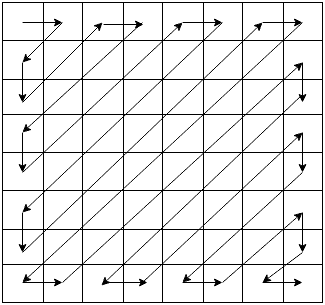
\includegraphics[width=0.3\textwidth]{zigzag.png}
        \caption{Zigzag Example}
    \end{figure}

    \begin{itemize}
     \item After quantization, many high-freqency coefficients become zero
     \item Zigzag scan reorders the $8\times8$ block into a 1D array
     \item Scanning pattern groups low-frequency coefficients first
     \item This creates long runs of zeros at the end of the sequence
    \end{itemize}
\end{frame}

\begin{frame}{Run Length Encoding (RLE)}
    \begin{itemize}
     \item Lossless compression step
     \item RLE encodes zigzag-scanned coefficients
     \item Represents sequences of zeros folowed by non-zero values
     \item DC components encoded as difference from previous DC component
     \item End of block encoded as (0,0)
    \end{itemize}

    \vspace{0.5cm}
    \textbf{Example:}
    \begin{center}
     Original: [42, 0, 0, 0, 7, 0, 0, 0, 0, 0, 0, 0, ...]\\
     RLE: [(0,42), (3,7), (0,0)]
    \end{center}

\end{frame}


\section{JPEG Decoding}

\begin{frame}{Decoding Process}
    \textbf{JPEG Decoding reverses the encoding steps:}
    \begin{enumerate}
     \item Parse the file header to extract \textbf{quantization tables}
     \item Decode \textbf{RLE} encoded data back to coefficient sequences
     \item Perform \textbf{inverse zigzag} scanning to reconstruct $8\times8$ blocks
     \item Multiply coefficients by their respective \textbf{quantization} table values
     \item Apply \textbf{Inverse DCT} to convert from frequency to spatial domain
     \item Restore original resolution for \textbf{Chroma channels}
     \item Convert from $\bm{Y'C_bC_r}$ to $\bm{RGB}$
    \end{enumerate}

\end{frame}


\section{Optimizations}

\begin{frame}{DCT Optimization: Separable 1D Transform}
    \textbf{Standard 2D DCT vs. Optimized Approach:}
    \begin{itemize}
     \item \textbf{Standard 2D DCT:} $O(N^4)$ complexity for $N \times N$ block
     \item \textbf{Separable 1D DCT:} $O(N^3)$ complexity - significant speedup!
    \end{itemize}

    \vspace{0.3cm}
    \textbf{Precomputed Cosine Table}
    \begin{itemize}
     \item Cosine values in DCT formula do not depend on pixel values
     \item Compute a table with all possible cosine values which could be used in DCT formula
    \end{itemize}

    \vspace{-0.3cm}
    $$\text{DCT}(i,j) = \cos\left(\frac{(2j+1) \cdot i \cdot \pi}{16}\right)$$

    \textbf{Separable Transform Process:}
    \begin{enumerate}
     \item \textbf{Row Transform:} $R_{DCT}(i,j) = \sum_{k=0}^{7}\text{pixel}(i,k) \cdot C(j) \cdot \text{DCT}(j,k)$
     \item \textbf{Column Transform:} $\text{DCT}(i,j) = \frac{1}{4} \sum_{k=0}^{7} R_{DCT}(k,j) \cdot C(i) \cdot \text{DCT}(i,k)$
    \end{enumerate}

\end{frame}

\begin{frame}{Additional Optimizations}
    \textbf{1. Multithreaded Channel Processing}
    \begin{itemize}
     \item Each color channel ($Y$,$C_b$,$C_r$) processed in separate thread
     \item Parallel execution for both encoding and decoding
     \item \textbf{Performance gain:} Up to $3\times$ speedup on multi-core systems
     \item Implementation: \texttt{pthred\_create()} for each channel, \texttt{pthread\_join()} to synchronize before final write
    \end{itemize}

    \vspace{0.3cm}
    \textbf{2. In-Place Memory Management}
    \begin{itemize}
     \item \textbf{Memory type casting:} Same buffer used for float$\rightarrow$int conversion
     \begin{itemize}
      \item DCT coefficients stored as \texttt{float}
      \item After quantization, same memory reinterpreted as \texttt{int32\_t}
     \end{itemize}
    \end{itemize}
\end{frame}

\section{Performance Evaluation}

\begin{frame}{Performance Evaluation}
    \textbf{Compression Efficiency:}
    \begin{itemize}
     \item Acheived 7:1 compression ratio on 24-bit BMP files at 75\% quality setting
    \end{itemize}

    \vspace{0.3cm}

    \textbf{Processing Speed Analysis:}
    \begin{itemize}
     \item \textbf{High-resolution image (5184x3456 pixels):}
     \begin{itemize}
      \item Compression: 0.7 seconds
      \item Decompression: 0.5 seconds
     \end{itemize}

     \item \textbf{Low-resolution image (218x241 pixels):}
     \begin{itemize}
      \item Compression: 0.003 seconds
      \item Decompression: 0.001 seconds
     \end{itemize}
    \end{itemize}

    \vspace{0.3cm}

    \textbf{Memory Management:}
    \begin{itemize}
     \item Memory leak analysis performed using Valgrind
     \item Zero memory leaks or errors detected
     \item Peak heap usage: 451 MB for high-resolution image processing
    \end{itemize}
\end{frame}

\section{References}

\begin{frame}{References}
    \footnotesize
    \begin{enumerate}
     \item \href{https://en.wikipedia.org/wiki/JPEG}{Wikipedia, JPEG}
     \item \href{https://www.baeldung.com/cs/jpeg-compression}{Baeldung, JPEG Compression Explained}
     \item \href{https://cs.stanford.edu/people/eroberts/courses/soco/projects/data-compression/lossy/jpeg/index.htm}{Stanford University, Lossy Data Compression: JPEG}
     \item \href{https://en.wikipedia.org/wiki/Discrete_cosine_transform}{Wikipedia, Discrete Cosine Transform}
    \end{enumerate}

\end{frame}

\end{document}
